\documentclass{beamer}
\usetheme{Berlin}
\usepackage{stmaryrd}
\usepackage{float}
\beamerdefaultoverlayspecification{<+->}

\makeatletter
\newsavebox{\@brx}
\newcommand{\llangle}[1][]{\savebox{\@brx}{\(\m@th{#1\langle}\)}%
  \mathopen{\copy\@brx\kern-0.5\wd\@brx\usebox{\@brx}}}
\newcommand{\rrangle}[1][]{\savebox{\@brx}{\(\m@th{#1\rangle}\)}%
  \mathclose{\copy\@brx\kern-0.5\wd\@brx\usebox{\@brx}}}
\makeatother

\expandafter\def\expandafter\insertshorttitle\expandafter{%
  \insertshorttitle\hfill%
  \insertframenumber\,/\,\inserttotalframenumber}

\title{Coded Computation: Straggler Mitigation in Distributed Matrix Multiplication\thanks{Yu et al., IEEE Transactions on Information Theory, 2020}}
\author{Ankit Kumar Misra \and Dhruva Dhingra}
\institute{EE 605: Error Correcting Codes, \\Autumn 2022, IIT Bombay}
\date{\today}

\begin{document}

\frame{\titlepage}

\begin{frame}{Distributed Matrix Multiplication}
\begin{itemize}
    \item Matrix multiplication is a fundamental operation in data analytics and machine learning applications.
    \item Often requires a lot more storage and computational power than a single machine can offer.
    \item This problem is solved by deploying the multiplication task over a large-scale distributed system, having several nodes.
\end{itemize}
\end{frame}

\begin{frame}{The Straggler's Delay Bottleneck}
\begin{itemize}
    \item But what if some nodes are slower than others?
    \item The slowest nodes, a.k.a. \textit{stragglers}, impose a latency bottleneck.
    \item Commonly tackled by adding redundant computations.
    \item Naturally, error correcting codes can be applied to introduce `efficient redundancy' in computation.
\end{itemize}
\end{frame}

\begin{frame}{Modelling the Problem}
\begin{itemize}
    \item Input matrices $A\in \mathbb{F}^{s\times r}$ and $B\in\mathbb{F}^{s\times t}$.
    \item One master node and $N$ worker nodes, each of which can store $1/pm$ fraction of $A$ and $1/pn$ fraction of $B$.
    \item Encoding functions $\mathbf{f} = (f_0,\dots,f_{N-1})$ and $\mathbf{g} = (g_0,\dots,g_{N-1})$, and class of decoding functions $\mathbf{d} = \{d_{\mathcal{K}}\}_{\mathcal{K}\subseteq \{0,1,\dots,N-1\}}$.
    \item Master sends $\tilde{A}_i = f_i(A)$ and $\tilde{B}_i = g_i(B)$ to worker $i$.
    \item Worker $i$ sends $\tilde{C}_i = \tilde{A}^T_i\tilde{B}_i$ to master.
    \item Master estimates $C$ using $\hat{C} = d_{\mathcal{K}}(\{\tilde{C}_i\}_{i\in\mathcal{K}})$ using $\tilde{C}_i$ values received from a subset $\mathcal{K}$ of workers.
    \item $k$-recoverable if $\hat{C}=C$ for all $\mathcal{K}$ s.t. $|\mathcal{K}|=k$.
    \item Recovery threshold $K(\mathbf{f}, \mathbf{g}, \mathbf{d})$ is smallest $k$ s.t. $k$-recoverable.
\end{itemize}
\end{frame}

\begin{frame}{Redundant Code}
    \begin{itemize}
        \item Divide $A \in \mathbb{F}^{s \times r}$ into $r_{1}$ matrices of size $\mathbb{F}^{s\times r / r_{1}}$. Divide $B \in \mathbb{F}^{s \times t}$ into $r_{2}$ matrices of size $\mathbb{F}^{s \times t / r_{2}}$. 
        \item Give each worker the task of computing the product of one submatrix of $A$ with another submatrix of $B$.
        \item There are $N$ workers and $r_{1} \times r_{2}$ unique computations. As soon as we have $r_{1} \times r_{2}$ unique results of the form $A^T_iB_j$, we can interpolate the complete matrix.
        \item Thus, the redundancy is $\dfrac{N}{r_{1} r_{2}}$
    \end{itemize}
\end{frame}

\begin{frame}{Linear Codes}
    \only<1->{\begin{align*}
        A = \begin{bmatrix}
            A_{0,0} & \dots & A_{0,m-1}\\
            \vdots & \ddots & \vdots\\
            A_{p-1,0} & \dots & A_{p-1,m-1}
        \end{bmatrix}, && B = \begin{bmatrix}
            B_{0,0} & \dots & B_{0,n-1}\\
            \vdots & \ddots & \vdots\\
            B_{p-1,0} & \dots & B_{p-1,n-1}
        \end{bmatrix}
    \end{align*}}
    \only<2->{\begin{align*}
        \tilde{A}_i = \sum_{j,k}A_{j,k}a_{ijk} && \tilde{B}_i = \sum_{j,k}B_{j,k}b_{ijk}
    \end{align*}}
    \only<3->{\begin{align*}
        \hat{C}_{j,k} = \sum_{i\in\mathcal{K}}\tilde{C}_ic_{ijk}
    \end{align*}}
\end{frame}

\begin{frame}{Entangled Polynomial Code}
    \begin{itemize}
        \item Assign a distinct $x_i\in\mathbb{F}$ to each worker $i$.
        \item Worker $i$ is given the following:
        \begin{align*}
            \tilde{A}_i = \sum_{j=0}^{p-1}\sum_{k=0}^{m-1}A_{j,k}x^{j+kp}_i && \tilde{B}_i = \sum_{j=0}^{p-1}\sum_{k=0}^{n-1}B_{j,k}x^{p-1-j+kpm}_i
        \end{align*}
        \item Worker $i$ returns 
        \begin{align*}
        \tilde{C}_i &= \tilde{A}_i^{T} \tilde{B}_i \\
        &= \sum_{j=0}^{p-1} \sum_{k=0}^{m-1} \sum_{j'=0}^{p-1} \sum_{k='0}^{n-1} A_{j,k}^{T} B_{j',k'} x_{i}^{(p-1 + j - j') + kp + k'pm}
        \end{align*}
    \end{itemize}
\end{frame}

\begin{frame}{Entangled Polynomial Code}
    \begin{itemize}
        \item $\tilde{C}_{i}$ is interpolation of polynomial $h(x)$ at $x = x_{i}$ where
        \[ h(x) = \sum_{j=0}^{p-1} \sum_{k=0}^{m-1} \sum_{j'=0}^{p-1} \sum_{k='0}^{n-1} A_{j,k}^{T} B_{j',k'} x^{(p-1 + j - j') + kp + k'pm} \]
        \item $C_{k, k'}$ is the coefficient of $(p - 1 + kp + k'pm)$-th degree term.
        \item Degree of $h(x)$ is $pmn + p - 2$. So, given evaluation of $h(x)$ at any distinct $pmn + p - 1$ points, we can find the coefficients of $h(x)$ which are the required submatrices of the result.
        \begin{theorem}
            $K_{\text{entangled-poly}} = pmn + p - 1$.
        \end{theorem}
    \end{itemize}
\end{frame}

\begin{frame}{Why are Entangled Polynomial Codes Important?}
    \begin{theorem}
        $K^*_{\text{linear}} = K_{\text{entangled-poly}}$.
    \end{theorem}

    \begin{theorem}
        If $\mathbb{F}$ is a finite field, then $\frac{1}{2}K_{\text{entangled-poly}} < K^* \leq K_{\text{entangled-poly}}$.
    \end{theorem}
\end{frame}

\begin{frame}{What we did}
    \begin{itemize}
        \item We implemented entangled polynomial codes and redundant codes in Python.
        \item Code at \url{https://github.com/ankitkmisra/Straggler-Mitigation-MatMul}.
        \item We simulated communication delays with two exponential distributions; a low-mean one for fast workers and a high-mean one for slow workers. ($p(x;\lambda) = \lambda e^{-\lambda x}$)
        \item A fraction $f < 1$ of workers were set to be slow.
        \item We observed computation times and errors in the final result, for both types of codes, by varying matrix sizes, number of partitions, number of workers, etc.
    \end{itemize}
\end{frame}

\begin{frame}{Practical Issues with Entangled Polynomial Code - Numerical Instability}
    \begin{itemize}
        \item \textbf{Interpolation Error} - Lagrange Interpolation is numerically very unstable. As soon as interpolation degree crosses 20, error starts rising very quickly (Runge's phenomenon\footnote{\url{https://en.wikipedia.org/wiki/Runge's_phenomenon}}).
        \item \textbf{Solution} - Use Chebyshev Nodes\footnote{\url{https://en.wikipedia.org/wiki/Chebyshev_nodes}} for evaluation points. 
        \begin{align*}
            x_k = \cos\left(\dfrac{2k-1}{2n}\pi\right)
        \end{align*}
    \end{itemize}
\end{frame}

\begin{frame}{Practical Issues with Entangled Polynomial Code - Numerical Instability}
    \begin{figure}[H]
        \centering
        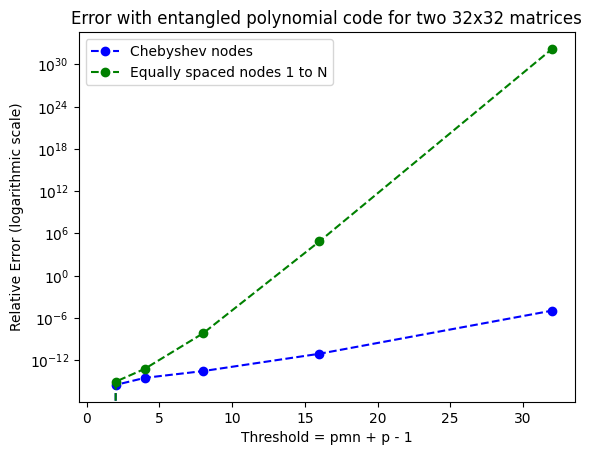
\includegraphics[scale=0.5]{error_vs_threshold.png}
        \caption{Caption}
    \end{figure}
\end{frame}

\begin{frame}{Practical Issues with Entangled Polynomial Code - Preprocessing Time}
    \begin{itemize}
        \item Encoding and Decoding for Entangled Polynomial Code is very expensive.
        \item While multiplying a matrix with a scalar and summing over the block matrices is not expensive, calculating $x_{i}^{\mathbf{J} + \mathbf{K}p}$ for $\tilde{A}_{i}$ and $x_{i}^{p-1-\mathbf{J}+\mathbf{K}pm}$ for $\tilde{B}_{i}$ is a very expensive operation.
        \item In fact, this preprocessing time (even for a single worker) soon begins to eclipse the time taken for matrix multiplcation at a single worker.
        \item Empirical analysis validates this result.
    \end{itemize}
\end{frame}

\begin{frame}{Practical Issues with Entangled Polynomial Code - Preprocessing Time}
    \begin{figure}[H]
        \centering
        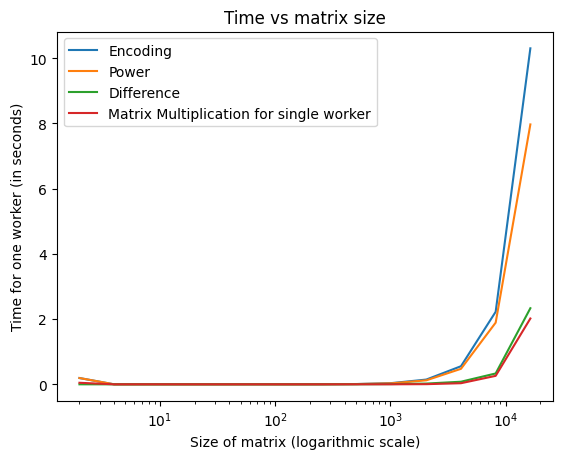
\includegraphics[scale=0.5]{encoding_time_single_worker_vs_matrix_size}
        \caption{Caption}
    \end{figure}
\end{frame}

\begin{frame}{Execution times: Polynomial code vs. Redundant code}
    \begin{figure}[H]
        \centering
        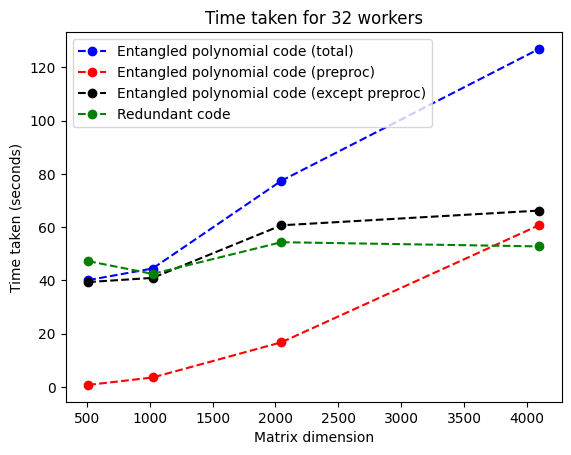
\includegraphics[scale=0.5]{time_vs_matsize.png}
        \caption{Caption}
    \end{figure}
\end{frame}

\begin{frame}{Conclusions}
    \begin{itemize}
        \item Entangled polynomial codes are extremely effective for reconstruction from a minimal number of responsive workers.
        \item But there are two problems:
        \begin{itemize}
            \item Interpolation introduces errors, which increase exponentially with the number of evaluation points used.
            \item Cost of preprocessing increases rapidly with matrix size, due to a large number of exponentiations, and causes a sharp increase in total computation time using entangled polynomial codes.
        \end{itemize}
        \item This renders entangled polynomial codes unfit for practical use, unless these issues are fixed.
    \end{itemize}
\end{frame}

\begin{frame}{}
    \Large{Thanks!}

    \bigskip

    \normalsize{Any questions?}
\end{frame}


\end{document}